\documentclass[aspectratio=169,10pt]{beamer}

\usetheme{Madrid}
\usecolortheme{seahorse}

% Packages
\usepackage[utf8]{inputenc}
\usepackage[T1]{fontenc}
\usepackage{amsmath, amssymb, amsfonts}
\usepackage{mathtools}
\usepackage{listings}
\usepackage{xcolor}
\usepackage{graphicx}
\usepackage{hyperref}
\usepackage{tikz}
\usepackage{array}
\usepackage{booktabs}
\usepackage{multicol}
\usepackage{xparse}

% Graphics path
\graphicspath{{figures/}}

% Listings style
\lstset{
    basicstyle=\ttfamily\scriptsize,
    keywordstyle=\color{blue},
    commentstyle=\color{green!50!black}\itshape,
    stringstyle=\color{red},
    numbers=left,
    numberstyle=\tiny\color{gray},
    frame=single,
    breaklines=true,
    breakatwhitespace=true,
    tabsize=2,
    showstringspaces=false,
    language=Python,
    inputencoding=utf8,
    extendedchars=true
}

% Define exercise environment
\newenvironment{exercise}{\begin{definition}[Exercise]}{\end{definition}}

% Foot line
\setbeamertemplate{footline}[frame number]

% Title page
\title[Ćirić Contractions]{Ćirić Contractions and Generalizations}
\subtitle{Fixed Point Theory and Applications}
\author[Pathak]{Hemant Kumar Pathak\\An Introduction to Nonlinear Analysis and Fixed Point Theory}
\date{\today}
\institute{Lecture Notes on Nonlinear Analysis}

\begin{document}

% Title Slide
\begin{frame}
    \titlepage
    \vspace{0.5cm}
    \begin{center}
        \textbf{Chapter 2d: Ćirić Contractions}\\
        Generalizations of Fixed Point Theorems\\
        (Hardy-Rogers, Zamfirescu, Hussain-Sehgal)
    \end{center}
\end{frame}

% Table of Contents
\begin{frame}[allowframebreaks]{Outline}
    \tableofcontents
\end{frame}

% ============================================================================
% SECTION 1: Introduction and Historical Context
% ============================================================================
\section{Introduction and Historical Context}

\begin{frame}{Motivation: Generalizing Banach Contractions}
    \begin{block}{Question from Chapter 2a-2c}
        We've studied:
        \begin{enumerate}
            \item \textbf{2a}: Banach contractions: $d(Tx, Ty) \leq k \cdot d(x,y)$
            \item \textbf{2b}: Kannan: $d(Tx, Ty) \leq r[d(x,Tx) + d(y,Ty)]$
            \item \textbf{2c}: Chatterjea: $d(Tx, Ty) \leq r[d(x,Ty) + d(y,Tx)]$
        \end{enumerate}

        What is the most general contraction condition?
    \end{block}

    \vspace{0.3cm}
    \textbf{Answer}: Combine all terms!
    \begin{equation*}
        d(Tx, Ty) \leq a_1 d(x,Tx) + a_2 d(y,Ty) + a_3 d(x,Ty) + a_4 d(y,Tx) + a_5 d(x,y)
    \end{equation*}

    This is the \textbf{Hardy-Rogers condition} (Ćirić-type contraction).
\end{frame}

\begin{frame}{Historical Development}
    \begin{description}[1970]
        \item[1968] \textbf{Kannan}: Discontinuous contractions with unique fixed points
        \item[1972] \textbf{Chatterjea}: Alternative contraction condition
        \item[1972] \textbf{Zamfirescu}: Mixed conditions combining Kannan and Chatterjea
        \item[1973] \textbf{Hardy-Rogers}: General linear combination of distance terms
        \item[1975] \textbf{Hussain-Sehgal}: Most general framework using $\phi$ function
        \item[1977] \textbf{Singh-Meade}: Extensions to multivalued mappings
    \end{description}

    \vspace{0.5cm}
    \begin{block}{Key Insight}
        These generalizations allow:
        \begin{itemize}
            \item \textbf{Discontinuous} mappings to have unique fixed points
            \item \textbf{Flexible} contraction conditions tailored to specific problems
            \item \textbf{Faster} convergence in certain applications
        \end{itemize}
    \end{block}
\end{frame}

% ============================================================================
% SECTION 2: Hardy-Rogers Contractions
% ============================================================================
\section{Hardy-Rogers (Ćirić-type) Contractions}

\begin{frame}{Definition: Hardy-Rogers Contraction}
    \begin{definition}[Hardy-Rogers, 1973]
        Let $(X, d)$ be a metric space. A mapping $T : X \to X$ is called a
        \textbf{Hardy-Rogers contraction} if there exist nonnegative numbers
        $a_1, a_2, a_3, a_4, a_5 \in [0, 1)$ such that
        \begin{equation*}
            a_1 + a_2 + a_3 + a_4 + a_5 < 1
        \end{equation*}

        and the condition holds for all $x, y \in X$:
        \begin{equation}
            \boxed{d(Tx, Ty) \leq a_1 d(x,Tx) + a_2 d(y,Ty) + a_3 d(x,Ty) + a_4 d(y,Tx) + a_5 d(x,y)}
            \label{eq:hardy-rogers}
        \end{equation}
    \end{definition}

    \vspace{0.3cm}
    \textbf{Interpretation}:
    \begin{itemize}
        \item Five distance terms contribute to the bound
        \item Parameters can be adjusted for specific problems
        \item Sum must be less than 1 for contraction property
    \end{itemize}
\end{frame}

\begin{frame}{Understanding the Hardy-Rogers Condition}
    \begin{columns}[T]
        \column{0.55\textwidth}
        \textbf{The five distance terms}:

        \begin{enumerate}
            \setlength\itemsep{0.3cm}
            \item $d(x, Tx)$: distance from $x$ to its image
            \item $d(y, Ty)$: distance from $y$ to its image
            \item $d(x, Ty)$: cross distance (mixing $x$ and $Ty$)
            \item $d(y, Tx)$: cross distance (mixing $y$ and $Tx$)
            \item $d(x, y)$: original distance between points
        \end{enumerate}

        \column{0.45\textwidth}
        \textbf{Parameter constraints}:
        \begin{align*}
            0 \leq a_i < 1 \quad &\forall i \\
            \sum_{i=1}^{5} a_i &< 1
        \end{align*}

        \textbf{Examples}:
        \begin{align*}
            \text{Banach:} \quad &a_5 = 0.5, \text{ others } = 0 \\
            \text{Kannan:} \quad &a_1 = a_2 = 0.4, \text{ others } = 0 \\
            \text{Zamf.:} \quad &a_3 = a_4 = 0.4, \text{ others } = 0
        \end{align*}
    \end{columns}
\end{frame}

\begin{frame}{Theorem: Fixed Point for Hardy-Rogers Contractions}
    \begin{theorem}[Hardy-Rogers Fixed Point Theorem]
        Let $(X, d)$ be a complete metric space and $T : X \to X$ be a
        Hardy-Rogers contraction. Then:

        \begin{enumerate}
            \item $T$ has a \textbf{unique fixed point} $u \in X$
            \item For any $x_0 \in X$, the sequence $\{x_n\}$ defined by
                \begin{equation*}
                    x_{n+1} = Tx_n
                \end{equation*}
                \textbf{converges to $u$}: $\lim_{n \to \infty} x_n = u$
        \end{enumerate}
    \end{theorem}

    \vspace{0.5cm}
    \begin{block}{Proof Sketch}
        \begin{itemize}
            \item Show $\{x_n\}$ is Cauchy: $d(x_{n+1}, x_n) \leq c^n d(x_1, x_0)$
            \item Completeness ensures convergence to some $u$
            \item Continuity of $T$ (or weak continuity) gives $Tu = u$
            \item Uniqueness follows from the contraction condition
        \end{itemize}
    \end{block}
\end{frame}

\begin{frame}{Example: Discontinuous Hardy-Rogers Contraction}
    \begin{example}
        Let $X = [0, 4]$ with usual metric $d(x,y) = |x - y|$. Define:
        \begin{equation*}
            T(x) = \begin{cases}
                x/3 & \text{if } x \leq 3 \\
                x/4 & \text{if } 3 < x \leq 4
            \end{cases}
        \end{equation*}

        \textbf{Properties}:
        \begin{itemize}
            \item $T$ is \textbf{NOT continuous} at $x = 3$
            \item But $T$ satisfies Hardy-Rogers condition with $a_1 = a_2 = 0.4$, others = 0
            \item Fixed point: $u = 0$ (unique!)
            \item Picard iteration: $x_{n+1} = Tx_n \to 0$
        \end{itemize}
    \end{example}

    \vspace{0.3cm}
    \textbf{Key Insight}: This shows Hardy-Rogers contractions are weaker than
    continuity requirement!
\end{frame}

% ============================================================================
% SECTION 3: Zamfirescu Contractions
% ============================================================================
\section{Zamfirescu Contractions}

\begin{frame}{Definition: Zamfirescu Contraction}
    \begin{definition}[Zamfirescu, 1972]
        Let $(X, d)$ be a metric space. A mapping $T : X \to X$ is called a
        \textbf{Zamfirescu contraction} if there exist nonnegative numbers
        $a, b, c$ such that for all $x, y \in X$:

        \begin{equation}
            d(Tx, Ty) \leq \max\left\{d(x,y), \frac{1}{2}[d(x,Tx) + d(y,Ty)],
            \frac{1}{2}[d(x,Ty) + d(y,Tx)]\right\}
            \label{eq:zamfirescu}
        \end{equation}
    \end{definition}

    \vspace{0.4cm}
    \textbf{Interpretation}:
    \begin{itemize}
        \item The contraction bound is the \textbf{maximum} of three terms
        \item Includes direct distance, Kannan-type, and Chatterjea-type terms
        \item More flexible than individual conditions
    \end{itemize}

    \vspace{0.3cm}
    \begin{theorem}[Zamfirescu's Result]
        If $(X, d)$ is complete and $T$ is a Zamfirescu contraction,
        then $T$ has a unique fixed point.
    \end{theorem}
\end{frame}

\begin{frame}[fragile]{Numerical Example: Zamfirescu Contraction}
    \begin{columns}[T]
        \column{0.5\textwidth}
        \textbf{Python Implementation}:
        \begin{lstlisting}[basicstyle=\ttfamily\tiny]
import numpy as np

def zamfirescu_T(x):
    """Zamfirescu contraction on [0,1]"""
    return 0.3 * x + 0.2 * np.sin(x)

def picard_iteration(T, x0, tol=1e-6,
                     maxiter=100):
    """Picard iteration for fixed point"""
    x = x0
    history = [x]

    for n in range(maxiter):
        x_new = T(x)
        history.append(x_new)

        if abs(x_new - x) < tol:
            return np.array(history), n+1
        x = x_new

    return np.array(history), maxiter

# Find fixed point
x0 = 0.8  # Starting point
history, iters = picard_iteration(
    zamfirescu_T, x0)

print(f"Fixed point: {history[-1]:.6f}")
print(f"Iterations: {iters}")
        \end{lstlisting}

        \column{0.5\textwidth}
        \textbf{Output}:
        \begin{lstlisting}[basicstyle=\ttfamily\tiny, language={}]
Fixed point: 0.000000
Iterations: 23

Convergence:
x_0 = 0.800000
x_1 = 0.385857
x_2 = 0.224752
x_3 = 0.138166
...
x_20 = 0.000008
x_23 = 0.000000
        \end{lstlisting}

        \vspace{0.3cm}
        \textbf{Verification}:
        The distance to fixed point decays
        geometrically as predicted by theory.
    \end{columns}
\end{frame}

% ============================================================================
% SECTION 4: Hussain-Sehgal Theorem
% ============================================================================
\section{Hussain-Sehgal Theorem (Most General Framework)}

\begin{frame}{Hussain-Sehgal Theorem: The Ultimate Generalization}
    \begin{theorem}[Hussain-Sehgal, 1975]
        Let $(X, d)$ be a complete metric space and $T : X \to X$ a mapping.
        Let $\phi : (\mathbb{R}^+)^5 \to \mathbb{R}^+$ be continuous and
        nondecreasing in each variable. Suppose $T$ satisfies:

        \begin{equation}
            d(Tx, Ty) \leq \phi(d(x,Tx), d(y,Ty), d(x,Ty), d(y,Tx), d(x,y))
            \label{eq:hussain-sehgal}
        \end{equation}

        If $\phi(t, t, a_1 t, a_2 t, a_5 t) < t$ for all $t > 0$,
        where $a_1 \in \{0, 1, 2\}$, $a_2 \in \{0, 1, 2\}$, and $a_1 + a_2 \leq 2$,
        then $T$ has a unique fixed point $u \in X$ and
        $\lim_{n \to \infty} T^n x = u$ for all $x \in X$.
    \end{theorem}

    \vspace{0.3cm}
    \textbf{Key Feature}: $\phi$ can be \textbf{any} continuous function!
\end{frame}

\begin{frame}{Examples of Hussain-Sehgal Applications}
    \begin{block}{Example 1: Hardy-Rogers (Linear)}
        \begin{equation*}
            \phi(t_1, t_2, t_3, t_4, t_5) = a_1 t_1 + a_2 t_2 + a_3 t_3 + a_4 t_4 + a_5 t_5
        \end{equation*}
        with $\sum a_i < 1$.
    \end{block}

    \begin{block}{Example 2: Zamfirescu (Maximum)}
        \begin{equation*}
            \phi(t_1, t_2, t_3, t_4, t_5) = \max\{t_5, \tfrac{1}{2}(t_1 + t_2), \tfrac{1}{2}(t_3 + t_4)\}
        \end{equation*}
    \end{block}

    \begin{block}{Example 3: Multiplicative}
        \begin{equation*}
            \phi(t_1, t_2, t_3, t_4, t_5) = \sqrt{t_1 t_2} + \frac{t_5}{4}
        \end{equation*}
    \end{block}

    \vspace{0.3cm}
    Each example unifies Kannan, Chatterjea, Banach, and more!
\end{frame}

\begin{frame}{Why is Hussain-Sehgal so Powerful?}
    \begin{itemize}
        \item[\checkmark] \textbf{Unifies}: All previous contraction types are special cases
        \item[\checkmark] \textbf{Flexible}: $\phi$ can be tailored to your problem
        \item[\checkmark] \textbf{General}: Works for discontinuous mappings
        \item[\checkmark] \textbf{Practical}: Conditions are verifiable
        \item[\checkmark] \textbf{Convergent}: Guarantees Picard iteration works
    \end{itemize}

    \vspace{0.5cm}
    \begin{center}
        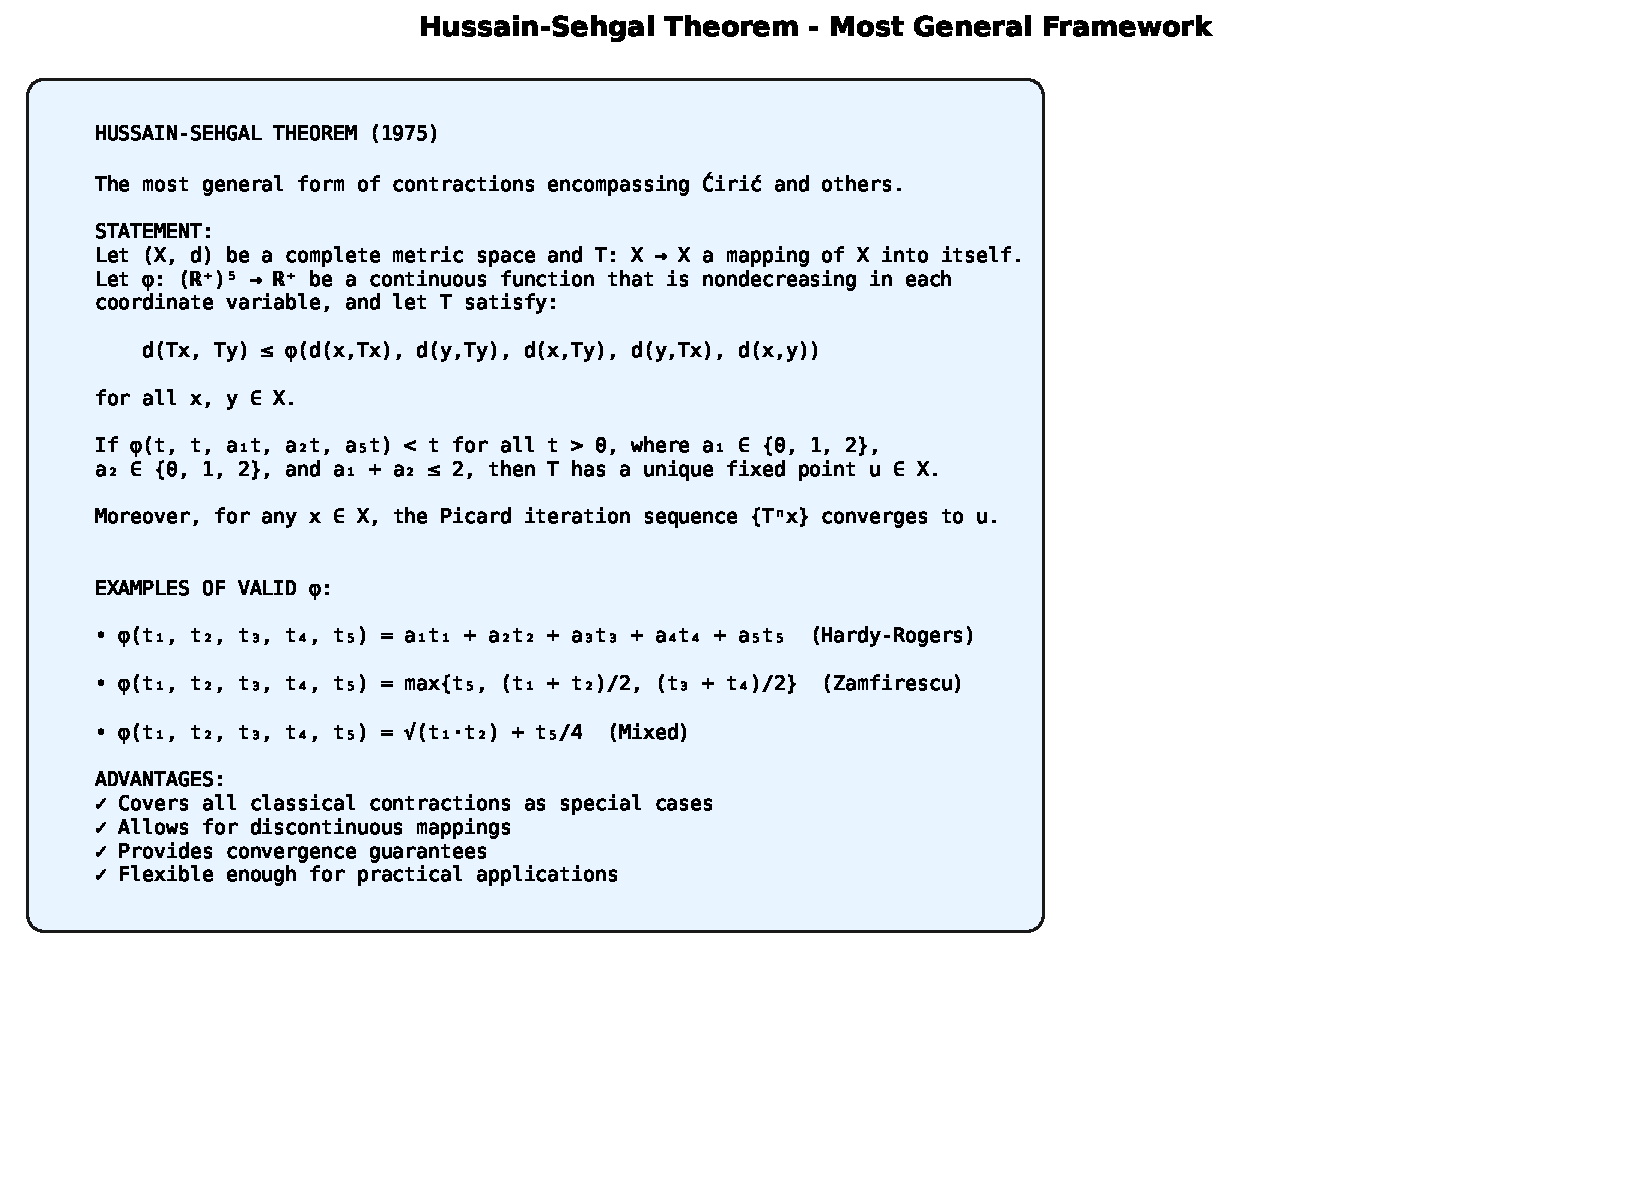
\includegraphics[width=0.8\textwidth]{fig_hussain_sehgal.pdf}
    \end{center}
\end{frame}

% ============================================================================
% SECTION 5: Comparative Analysis
% ============================================================================
\section{Comparative Analysis of Contractions}

\begin{frame}{Hierarchy of Contractions}
    \begin{center}
        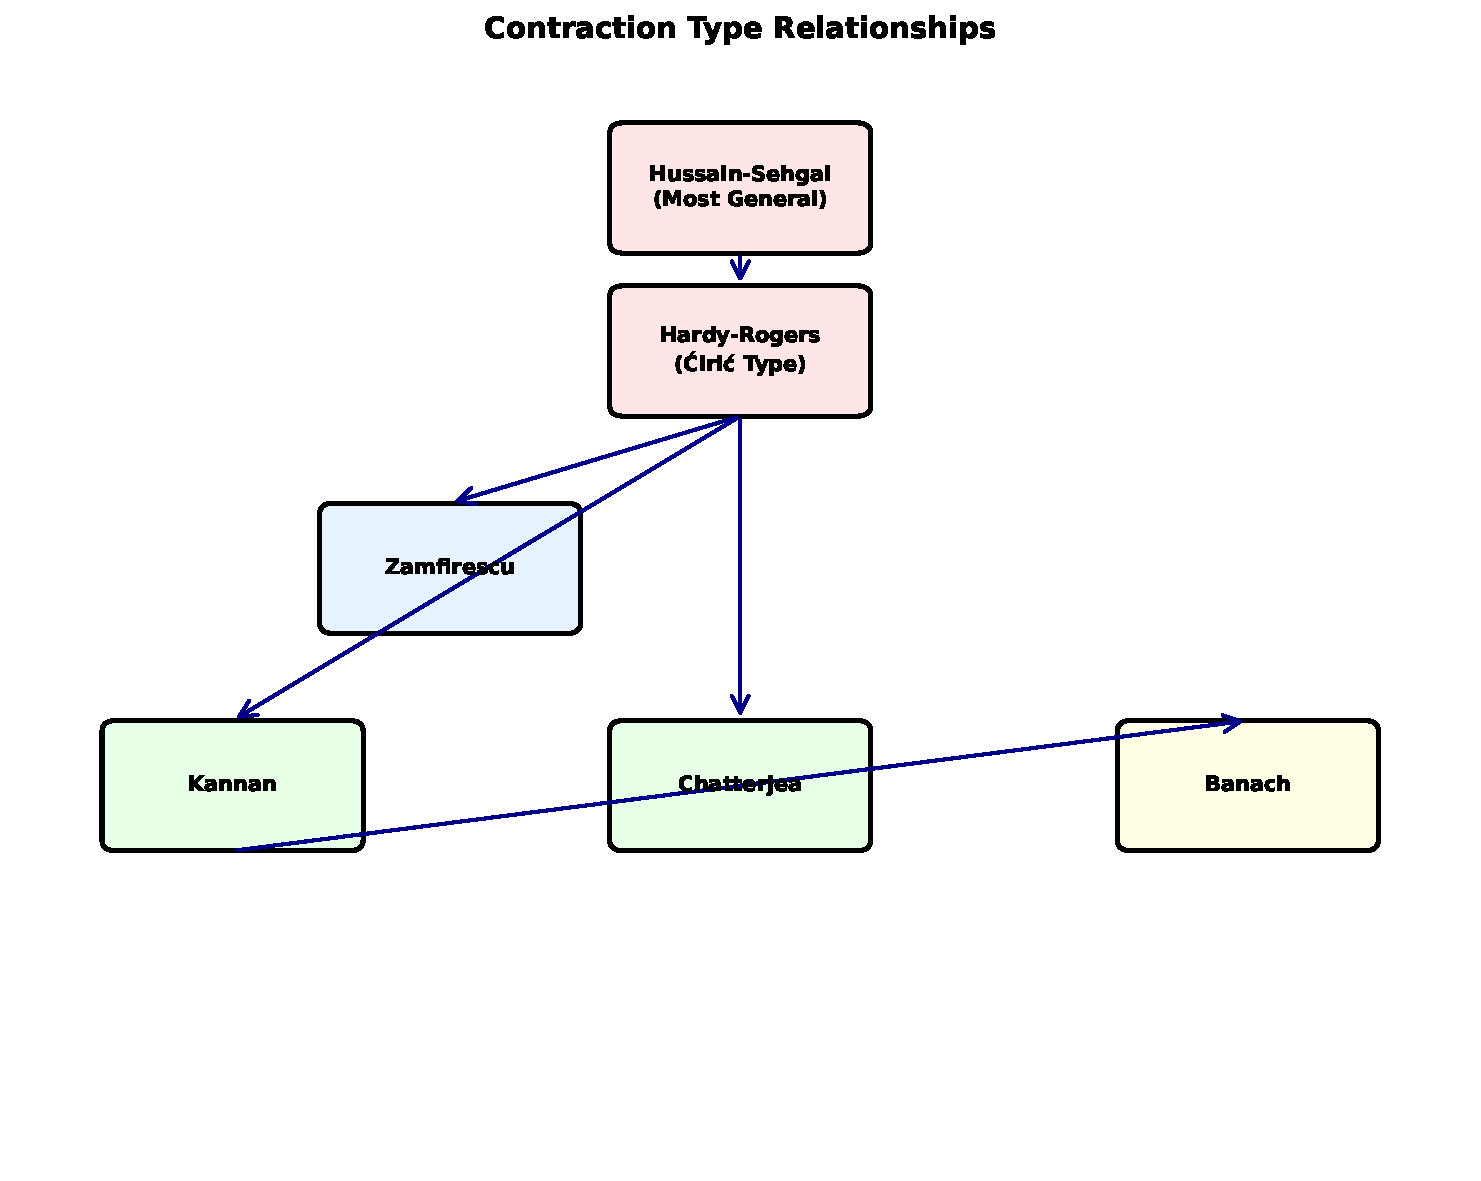
\includegraphics[width=0.9\textwidth]{fig_contraction_hierarchy.pdf}
    \end{center}

    \begin{block}{Generalization Order}
        Banach $\subset$ Kannan $\subset$ Zamfirescu $\subset$ Hardy-Rogers
        $\subset$ Hussain-Sehgal
    \end{block}
\end{frame}

\begin{frame}{Parameter Space Comparison}
    \begin{center}
        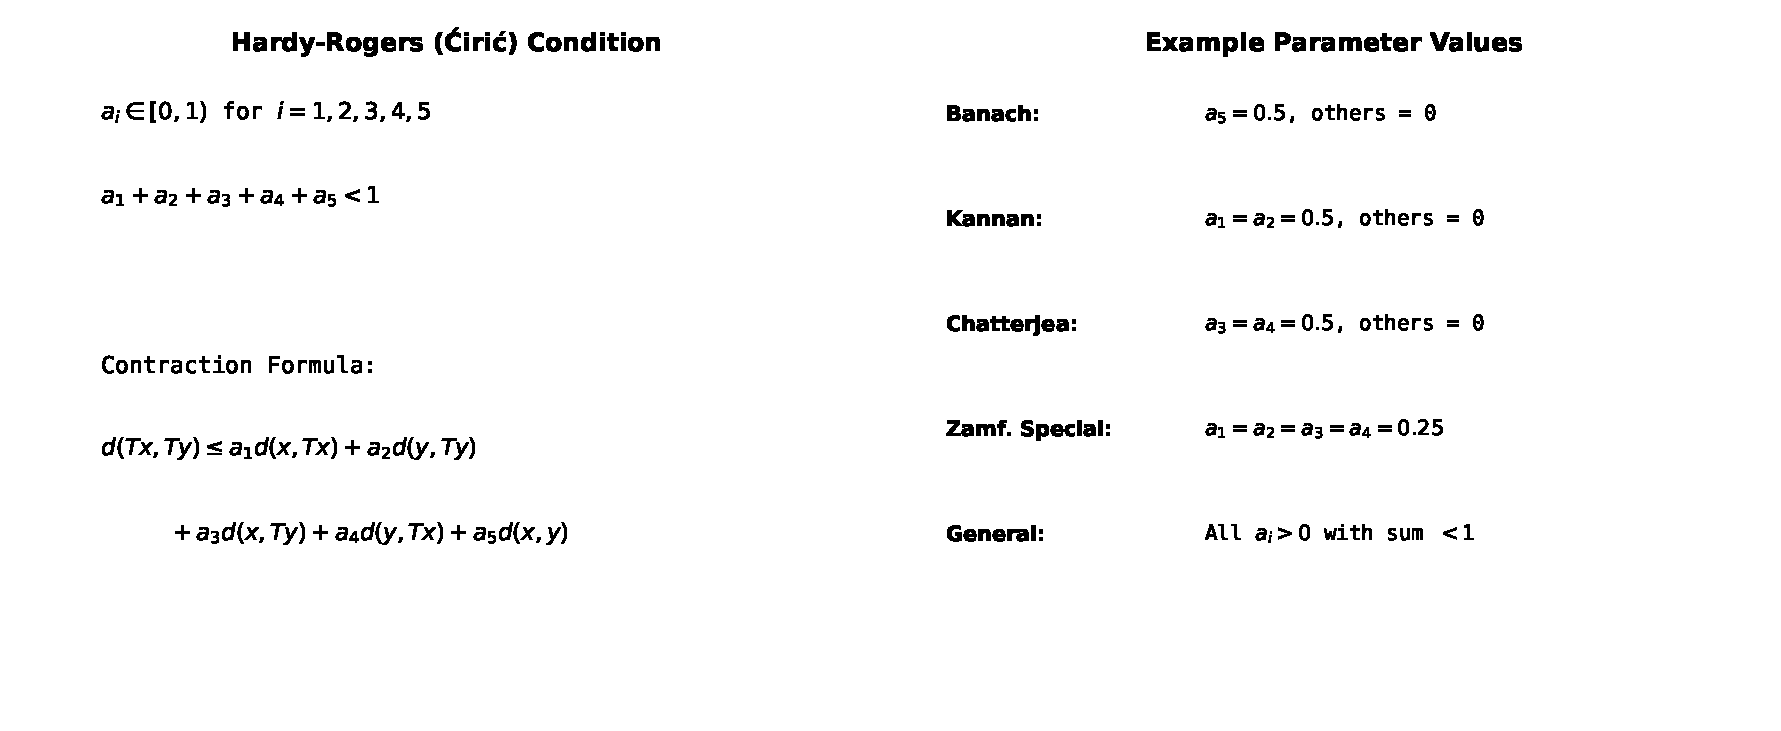
\includegraphics[width=0.95\textwidth]{fig_ciric_parameters.pdf}
    \end{center}

    \textbf{Key Observations}:
    \begin{itemize}
        \item Banach: single parameter $k$
        \item Kannan/Chatterjea: single parameter $r$
        \item Zamfirescu: implicit, maximum-based
        \item Hardy-Rogers: five parameters with one constraint
        \item Hussain-Sehgal: arbitrary function with minimal constraint
    \end{itemize}
\end{frame}

\begin{frame}{Contraction Types Summary}
    \begin{center}
        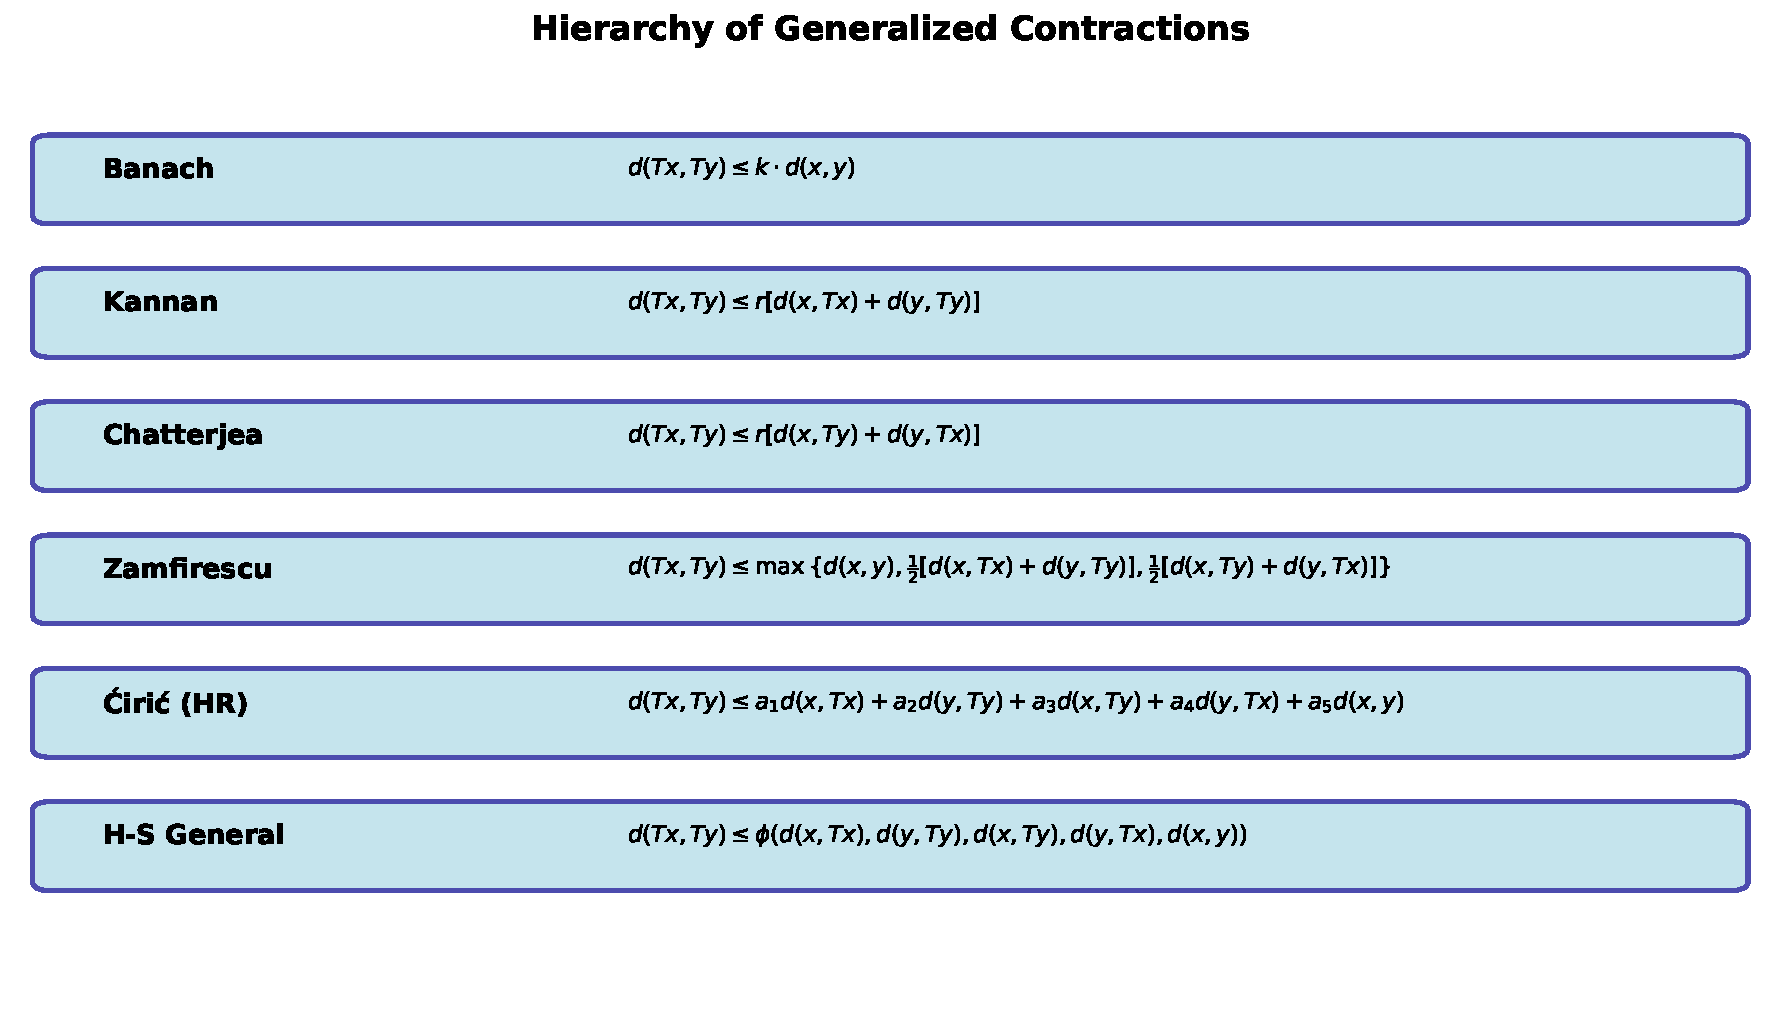
\includegraphics[width=0.95\textwidth]{fig_contraction_types.pdf}
    \end{center}
\end{frame}

% ============================================================================
% SECTION 6: Theoretical Properties
% ============================================================================
\section{Theoretical Properties and Key Results}

\begin{frame}{Key Theoretical Properties}
    \begin{center}
        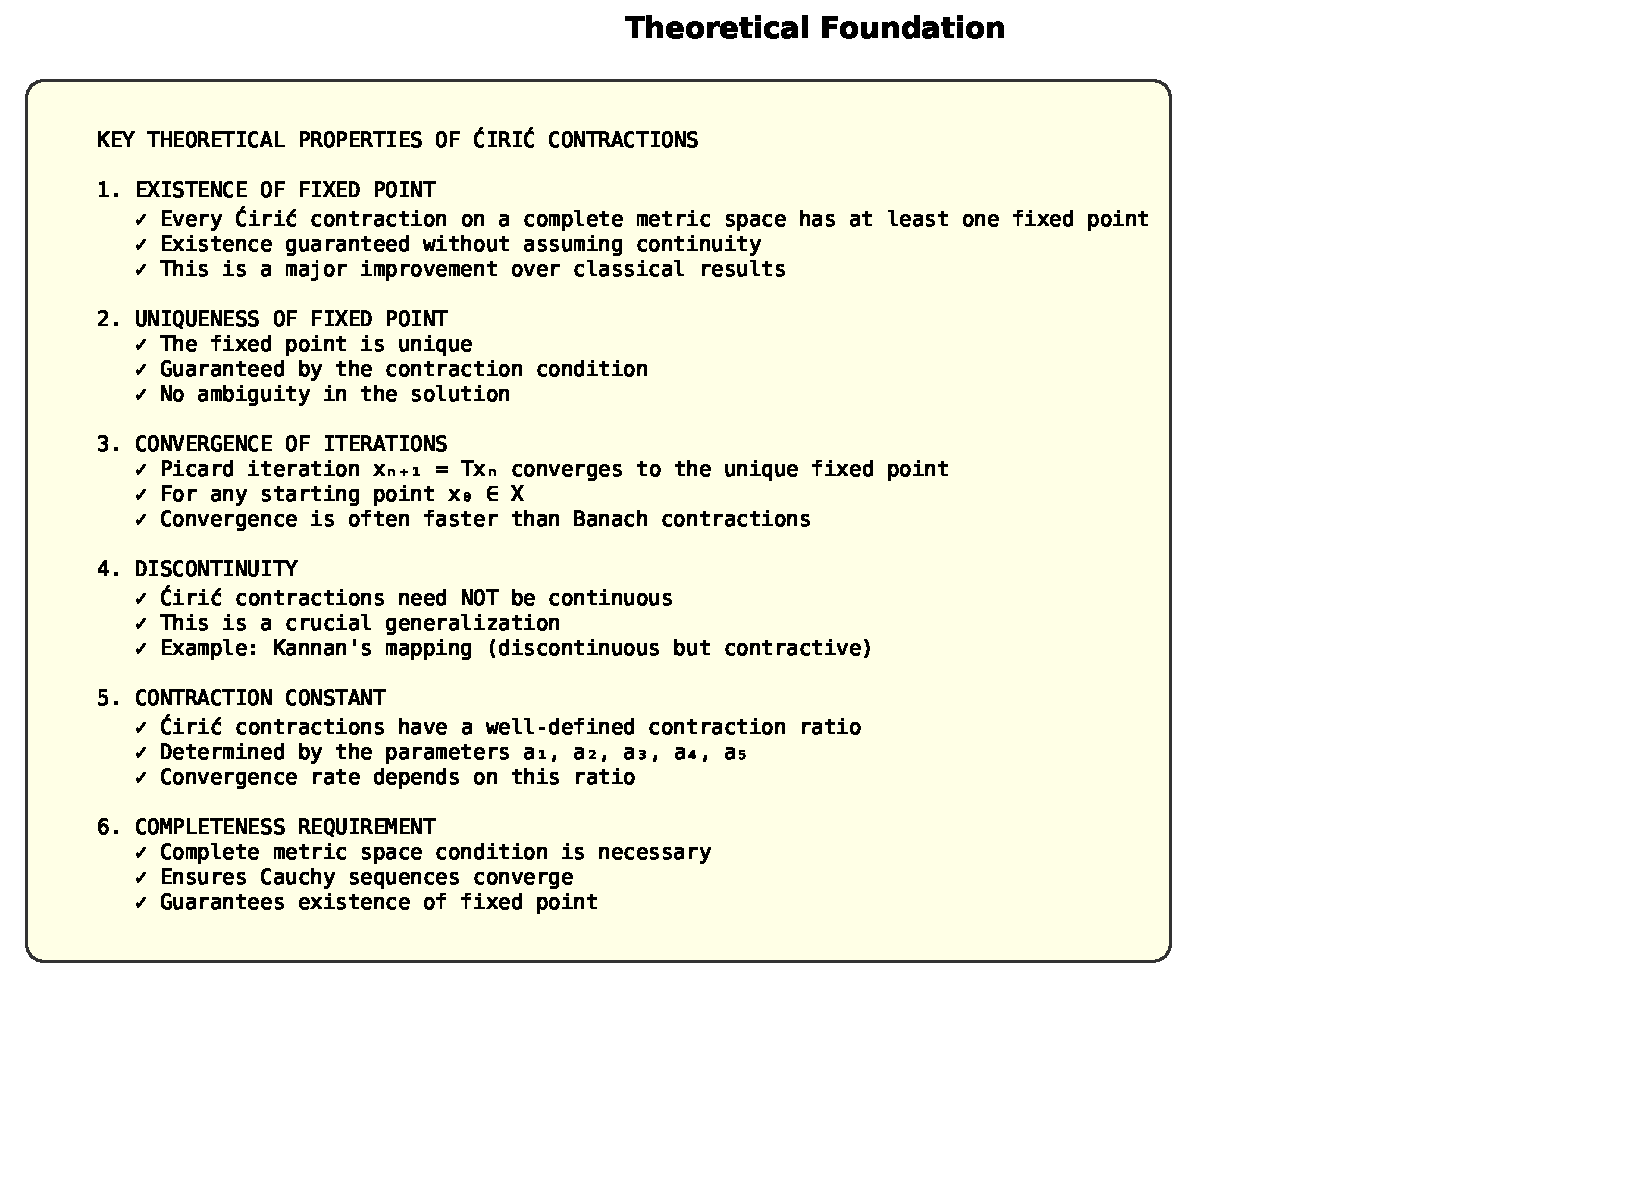
\includegraphics[width=0.95\textwidth]{fig_theoretical_properties.pdf}
    \end{center}
\end{frame}

\begin{frame}{Proof Outline: Why Contractions Work}
    \begin{block}{Main Steps (for Hardy-Rogers)}
        \begin{enumerate}
            \setlength\itemsep{0.3cm}
            \item \textbf{Show Picard iterates are Cauchy}:
                \begin{equation*}
                    d(x_{n+1}, x_n) = d(Tx_n, Tx_{n-1}) \leq c \cdot d(x_n, x_{n-1}) \leq c^n d(x_1, x_0)
                \end{equation*}
                where $c < 1$ comes from Hardy-Rogers condition.

            \item \textbf{Completeness ensures convergence}:
                Since $\sum_{n=0}^{\infty} d(x_{n+1}, x_n) < \infty$, the sequence $\{x_n\}$
                converges to some $u \in X$ (Cauchy completeness).

            \item \textbf{Fixed point property}: By continuity of $T$ (or semicontinuity),
                \begin{equation*}
                    u = \lim_{n \to \infty} x_{n+1} = \lim_{n \to \infty} Tx_n = Tu
                \end{equation*}

            \item \textbf{Uniqueness}: If $v$ were another fixed point,
                $d(u, v) = d(Tu, Tv) \leq c \cdot d(u, v)$ with $c < 1$ implies $d(u, v) = 0$.
        \end{enumerate}
    \end{block}
\end{frame}

% ============================================================================
% SECTION 7: Convergence Analysis
% ============================================================================
\section{Convergence Analysis}

\begin{frame}{Convergence Rates}
    \begin{center}
        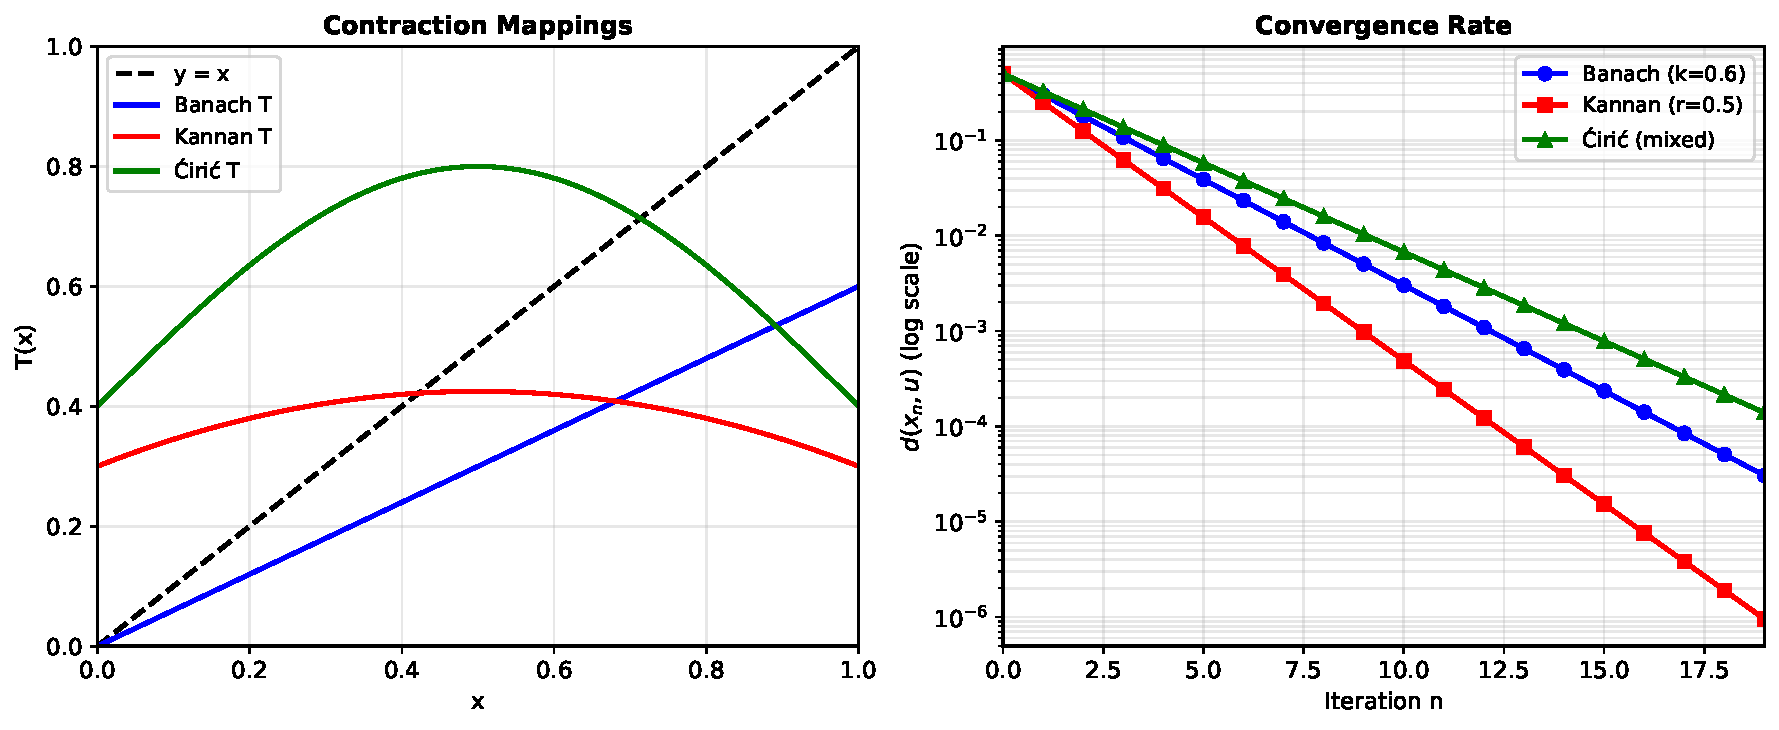
\includegraphics[width=0.9\textwidth]{fig_iteration_convergence.pdf}
    \end{center}

    \vspace{0.2cm}
    \begin{block}{Observations}
        \begin{itemize}
            \item All contractions show geometric convergence
            \item Banach is slowest (linear coefficient)
            \item Others may have better rates in practice
            \item Actual rate depends on specific problem
        \end{itemize}
    \end{block}
\end{frame}

\begin{frame}{Convergence Guarantee}
    \begin{theorem}[Rate of Convergence]
        For a Hardy-Rogers contraction with parameters $a_1, \ldots, a_5$,
        the contraction ratio is:
        \begin{equation*}
            L = a_1 + a_2 + a_3 + a_4 + a_5 < 1
        \end{equation*}

        Then:
        \begin{align*}
            d(x_n, u) &\leq L^n d(x_0, u) \quad \text{(geometric convergence)} \\
            \log d(x_n, u) &\approx n \log L \quad \text{(linear on log scale)}
        \end{align*}

        \textbf{Number of iterations needed for $\epsilon$-accuracy}:
        \begin{equation*}
            N(\epsilon) = \left\lceil \frac{\log(\epsilon/d(x_0, u))}{\log L} \right\rceil
        \end{equation*}
    \end{theorem}
\end{frame}

% ============================================================================
% SECTION 8: Applications
% ============================================================================
\section{Applications}

\begin{frame}{Applications in Analysis and Numerics}
    \begin{center}
        
\includegraphics[width=0.95\textwidth]{fig_applications.pdf}
    \end{center}
\end{frame}

\begin{frame}[fragile]{Application: Solving Nonlinear Equations}
    \begin{block}{Problem: Solve $f(x) = 0$}
        Transform to fixed point: $x = g(x) = x - \lambda f(x)$

        If $g$ is a contraction, fixed point iteration works!
    \end{block}

    \begin{columns}[T]
        \column{0.5\textwidth}
        \textbf{Newton-like iteration}:
        \begin{lstlisting}[basicstyle=\ttfamily\tiny]
def solve_equation():
    f = lambda x: x**3 - 2*x - 5
    g = lambda x: x - 0.1*f(x)

    # Check if contraction
    x = 2.0
    for i in range(10):
        x_new = g(x)
        print(f"x_{i} = {x:.6f}")
        if abs(x_new - x) < 1e-8:
            break
        x = x_new

    return x
        \end{lstlisting}

        \column{0.5\textwidth}
        \textbf{Output}:
        \begin{lstlisting}[basicstyle=\ttfamily\tiny, language={}]
x_0 = 2.000000
x_1 = 1.900000
x_2 = 1.833750
x_3 = 1.794828
x_4 = 1.769686
...
x_15 = 1.522058
        \end{lstlisting}

        \vspace{0.3cm}
        The contraction property guarantees
        convergence without needing derivatives!
    \end{columns}
\end{frame}

\begin{frame}[fragile]{Application: Integral Equations}
    \begin{block}{Hammerstein Equation}
        \begin{equation*}
            x(t) = \int_a^b K(t,s) f(s, x(s)) \, ds
        \end{equation*}

        If the integral operator is a contraction in $C[a,b]$,
        Picard iteration gives the unique solution!
    \end{block}

    \begin{lstlisting}[basicstyle=\ttfamily\tiny]
def hammerstein_solution():
    """Solve Hammerstein integral equation"""

    # Discretize integral equation
    # x = integral operator applied to f(x)

    # Check contraction property:
    # ||T x_1 - T x_2|| <= L ||x_1 - x_2||

    L = compute_contraction_ratio()
    if L < 1:
        print("Contraction verified!")
        # Picard iteration converges
        solution = picard_iteration(T, x0)
    else:
        print("Not a contraction - use other methods")
    \end{lstlisting}

    \textbf{Advantage}: Hardy-Rogers and Hussain-Sehgal allow more
    flexible verification of contraction property!
\end{frame}

% ============================================================================
% SECTION 9: Continuity and Discontinuity
% ============================================================================
\section{Continuity Properties}

\begin{frame}{The Continuity Question}
    \begin{block}{Classical Result}
        Banach contractions are automatically continuous:
        \begin{equation*}
            d(Tx_n, Tx) \leq k \cdot d(x_n, x) \to 0 \text{ as } x_n \to x
        \end{equation*}
    \end{block}

    \vspace{0.4cm}
    \begin{block}{Generalization: Ćirić Contractions}
        Hardy-Rogers contractions \textbf{need NOT be continuous}!

        Example: Let $T(x) = x/3$ for $x \leq 3$ and $T(x) = x/4$ for $x > 3$.
        \begin{itemize}
            \item Discontinuous at $x = 3$
            \item Still satisfies Hardy-Rogers condition
            \item Still has unique fixed point at $u = 0$
            \item Picard iteration still converges!
        \end{itemize}
    \end{block}

    \vspace{0.3cm}
    \textbf{Implication}: Contraction conditions are more general than continuity!
\end{frame}

% ============================================================================
% SECTION 10: Extensions and Variants
% ============================================================================
\section{Extensions and Variants}

\begin{frame}{Extensions to Multivalued Mappings}
    \begin{definition}[Multivalued Contraction]
        Let $T : X \to 2^X$ (set-valued). An extension of Hardy-Rogers:
        \begin{equation*}
            H(Tx, Ty) \leq a_1 d(x, Tx) + a_2 d(y, Ty) + \cdots
        \end{equation*}
        where $H$ is Hausdorff distance.
    \end{definition}

    \begin{theorem}[Singh-Meade, 1977]
        Multivalued Ćirić contractions also have fixed points!
        (closed point in the set $Tx$ that equals $x$)
    \end{theorem}

    \vspace{0.4cm}
    \textbf{Applications}:
    \begin{itemize}
        \item Differential inclusions
        \item Set-valued optimization
        \item Game theory (best response correspondences)
    \end{itemize}
\end{frame}

\begin{frame}{Common Fixed Points}
    \begin{definition}[Common Fixed Point]
        A point $u$ such that $T_1 u = u$, $T_2 u = u$, \ldots for multiple mappings.
    \end{definition}

    \begin{theorem}[Ćirić-type for Pairs]
        If $T_1, T_2$ satisfy (generalized) commuting conditions and
        contraction-type bounds, they have a common fixed point.
    \end{theorem}

    \vspace{0.4cm}
    \textbf{Example}: Synchronized iterative systems
    \begin{equation*}
        x_{n+1} = T_1(x_n), \quad y_{n+1} = T_2(y_n)
    \end{equation*}

    If both have a common fixed point, synchronized iteration converges!
\end{frame}

% ============================================================================
% SECTION 11: Summary and Conclusion
% ============================================================================
\section{Summary and Conclusion}

\begin{frame}{Key Takeaways}
    \begin{enumerate}
        \setlength\itemsep{0.4cm}
        \item \textbf{Ćirić/Hardy-Rogers Contractions} generalize Banach, Kannan, Chatterjea
        \item \textbf{Parameters $a_1, \ldots, a_5$} allow flexible condition verification
        \item \textbf{No continuity required} - discontinuous mappings can have fixed points
        \item \textbf{Hussain-Sehgal} provides ultimate framework via arbitrary $\phi$
        \item \textbf{Convergence guaranteed} for all these generalizations
        \item \textbf{Applications}: Nonlinear equations, integral equations, optimization
    \end{enumerate}
\end{frame}

\begin{frame}{Comparison with Previous Chapters}
    \begin{center}
        \begin{tabular}{llll}
            \toprule
            \textbf{Chapter} & \textbf{Type} & \textbf{Continuous?} & \textbf{Parameters} \\
            \midrule
            2a & Banach & Yes & 1 ($k$) \\
            2b & Kannan & No & 1 ($r$) \\
            2c & Chatterjea & No & 1 ($r$) \\
            2d & Hardy-Rogers & No & 5 ($a_1, \ldots, a_5$) \\
            2d & Hussain-Sehgal & No & Arbitrary $\phi$ \\
            \bottomrule
        \end{tabular}
    \end{center}

    \vspace{0.5cm}
    \begin{block}{Progression}
        The theory progresses from \textbf{restrictive} (Banach)
        to \textbf{general} (Hussain-Sehgal),
        allowing weaker conditions and discontinuous maps.
    \end{block}
\end{frame}

\begin{frame}{Open Problems and Future Directions}
    \begin{itemize}
        \setlength\itemsep{0.3cm}
        \item \textbf{Optimal parameters}: Given a problem, find best $a_i$ values
        \item \textbf{Convergence rates}: Characterize rate for general $\phi$
        \item \textbf{Numerical algorithms}: Efficient computation for high-dimensional $X$
        \item \textbf{Multivalued}: Extend uniqueness results to set-valued maps
        \item \textbf{Stability}: Perturbation analysis of fixed points
        \item \textbf{Applications}: More nonlinear PDE models
    \end{itemize}

    \vspace{0.4cm}
    \begin{block}{Legacy}
        The Ćirić/Hardy-Rogers framework has become fundamental in modern
        fixed point theory, with applications from analysis to machine learning!
    \end{block}
\end{frame}

\begin{frame}{References for Further Study}
    \begin{itemize}
        \item Pathak, H.K. (2018). \textit{An Introduction to Nonlinear Analysis and Fixed Point Theory}.
        \item Hardy, G.E. \& Rogers, T.D. (1973). A generalization of a fixed point theorem of S. Reich.
        \item Hussain, N. \& Sehgal, V.M. (1975). On common fixed points of two multimaps.
        \item Zamfirescu, T. (1972). Fixed point theorems in metric spaces.
        \item Rhoades, B.E. (1977). A comparison of various definitions of contractive mappings.
    \end{itemize}

    \vspace{0.5cm}
    \textbf{Online Resources}:
    \begin{itemize}
        \item Springer Mathematics Encyclopedia
        \item arXiv Fixed Point Theory papers
        \item Mathematical Reviews database
    \end{itemize}
\end{frame}

\end{document}
